\chapter{Referencial teórico}

Este capitulo apresenta os temas necessários para o desenvolvimento desse estudo e que devem ser tratados mais profundamente já que afetam o diretamente o foco principal do trabalho. Este capitulo foi estruturado em 4 tópicos, a saber: informações sobre o padrão 802.11 e as faixas utilizadas por ele, interferência de ondas, a tecnologia VLC e o projeto OpenVLC.

\section{Padrão IEEE 802.11}

Quando os computadores receberam transmissores e receptores de rádio varias empresas começaram a comercializar LANs sem fios, porém não havia uma padronização para a comunicação, ou seja, um computador equipado com um rádio da marca \emph{X} não era compatível com o computador equipado com o rádio da marca \emph{Y}. Diante deste problema surgiu a necessidade de se criar um padrão para as LANs sem fios, assim o comitê do IEEE criou o padrão 802.11 mais conhecido como \textit{wifi} \cite{tanenbaum}.

\subsection{Faixas 2.4Ghz e 5Ghz}

As faixas de radio que o \textit{wifi} utiliza são as faixas de 2,4GHz e 5GHz, as duas bandas não necessitam de licença para a sua utilização contudo os aparelhos devem limitar a sua potência para permitir que diferentes dispositivos coexistam. Como a utilização da faixa é livre é muito provável que os equipamentos de \textit{wifi} tenham que lidar constantemente com interferências \cite{tanenbaum}.

\section{Interferência de Ondas}

Se duas ondas senoidais de mesmo comprimento de onda são propagadas em uma corda no mesmo sentido mas estão defasadas, ou seja os picos estão alinhados com o vales da outra, elas se cancelam mutuamente e o deslocamento é zero. Este fenômeno chamados de interferência \cite{fisica}. 

\begin{figure}[!htbp]
  \caption{Demonstração das ondas resultantes}
  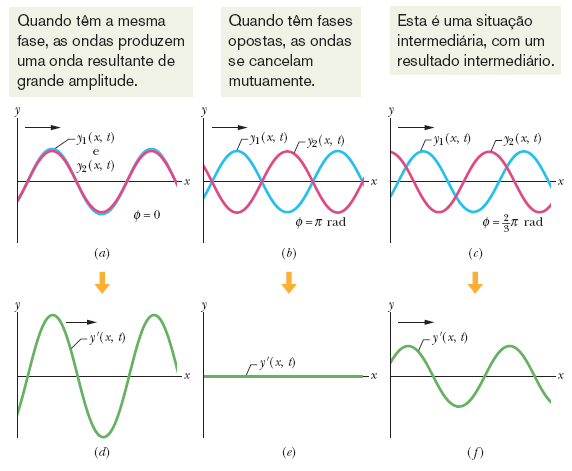
\includegraphics[scale=0.5]{images/ondas_interferencia.png}
  \legend{Fonte: \citeonline{fisica}}
  \label{fig:ondas_inter}
\end{figure}


\section{Visible Light Communication (VLC)}

Nesta seção sera apresentado o que é o VLC e conceitos relacionados ao tema, como a aplicações, vantagens e desvantagens e as formas de se modular a informação pra que seja possivel existir uma comunicação.

\subsection{O que é o VLC?}

Sistemas VLC são caracterizados por se comunicar utilizando a luz visível para modular as informações, ou seja, são utilizadas ondas que estão na faixa de 390nm a 700nm. Embora a luz visível seja usada para comunicação, o objetivo é que a transmissão seja imperceptível para o usuário, de modo que se assemelhe apenas a iluminação comum de uma lâmpada \cite{matheus2017comunicaccao}.

\begin{figure}[!htbp]
  \caption{O espectro eletromagnético}
  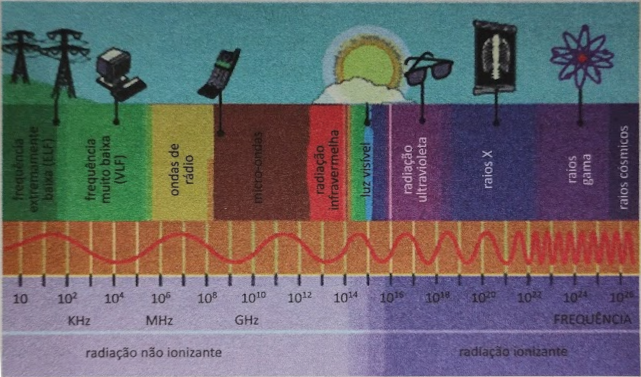
\includegraphics[scale=0.65]{images/espectro_eletromagnetico.png}
  \legend{Fonte: \citeonline{fisica}}
  \label{fig:espectro_eletromagnetico}
\end{figure}

\subsection{Aplicações}

A tecnologia do VLC pode ser utilizada de diversas formas como redes sem fio domesticas, pode ser utilizado para serviços de localização interna, já que o sinal de GPS não atravessa paredes. Também pode ser utilizado em locais onde ondas de radio não são muito desejáveis como cabines de avião e em hospitais \cite{matheus2017comunicaccao}. 

\subsection{Vantagens}

Dentre as diversas vantagens do VLC é o baixo consumo de energia, já que utiliza de lampadas de leds que consomem pouca energia, reduzindo em ate 75\% o consumo se comparado com outras lampadas. Outra vantagem proporcionada pelo uso de leds é a redução de custo já que são mais baratos e altamente duráveis, não necessitando de trocas frequentes \cite{matheus2017comunicaccao}.

Também notasse vantagem em relação a segurança como a luz não atravessa meios opacos dificultando para o invasor interceptar o sinal sem ser percebido, já que demandaria que estivesse no mesmo local de origem do sinal \cite{conceiccao2015comunicaccao}.

\subsection{Desvantagens}

Mesmo que a tecnologia VLC seja inovadora e que apresenta vantagens também existem algumas desvantagens, \citeauthoronline{matheus2017comunicaccao} e \citeauthoronline{conceiccao2015comunicaccao} citam algumas:

\begin{itemize}
  \item Pequeno alcance.
  \item Sujeito a interrupções devido a algum objeto que esta na frente do receptor.
  \item O desempenho pode ser prejudicado se houver diversas de luz no mesmo ambiente, gerando interferência.
\end{itemize}

\subsection{Modulação}

\subsubsection{On-Off Keying (OOK)}

Esta forma de modulação transmite os bits acendendo e apagando a lampada, mas também é possivel somente reduzir a intensidade da luz para representar o bit 0, já que no caso de se houver a transmissão de um byte \emph{100001} a lampada ficaria desligada por muito tempo, assim afetando a percepção do usuário \cite{matheus2017comunicaccao}.

\subsubsection{Color Shift Keying (CSK)}

O sinal é modulado através da intensidade de 3 cores, sendo elas vermelho, verde e azul, essas três cores juntas geram a luz branca. Como cita \citeauthoronline{matheus2017comunicaccao} a modulação OOK possui taxas de envio muito baixas por isso esta modulação foi proposta especificamente para o VLC \cite{matheus2017comunicaccao}. 

A modulação é feita relacionando cada bit a uma cor das coordenadas CIE 1931, \citeauthoronline{Abraham_2016} explica que é um sistema de correspondência de cores que permite especificar numericamente uma cor com o objetivo de reproduzi-la com precisão. Existem 7 bandas de comprimento que podem ser selecionadas para determinar as vértices de um triângulo no qual os pontos da constelação dos símbolos CSK estão. Cada ponto selecionado determina a intensidade da cor no led RGB \cite{matheus2017comunicaccao}.

\begin{figure}[!htbp]
  \caption{Diagrama de cromaticidade CIE 1931}
  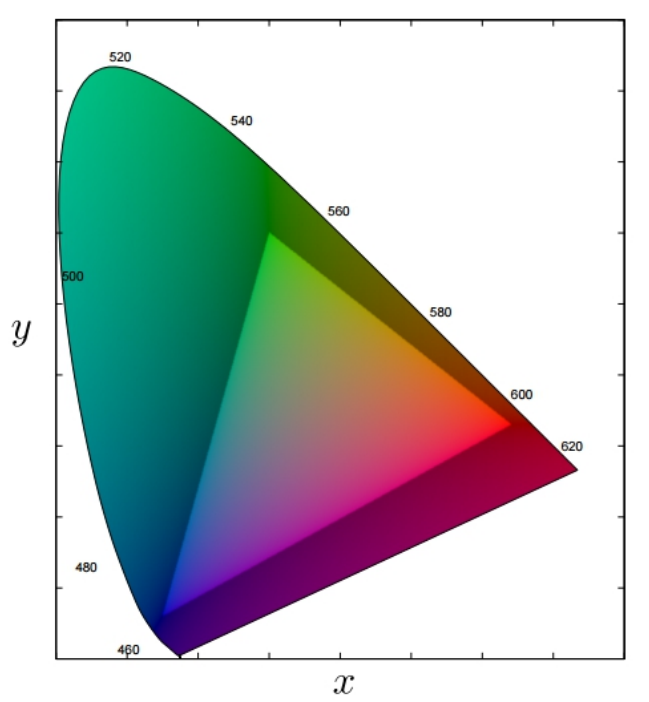
\includegraphics[scale=0.4]{images/csk.png}
  \legend{Fonte: \apudonline{monteiro}{matheus2017comunicaccao} }
  \label{fig:}
\end{figure}


\section{OpenVLC}

O OpenVLC é uma plataforma \textit{open source} baseada em  Linux e na plataforma Beagle Bone Black (BBB), projetada para ser de baixo custo e ser utilizada em pesquisas de redes VLC. O projeto consiste em um \textit{hardware} para a transmissão e recepção e sua implementação de \textit{software} atua na camada de enlace \cite{OpenVLCB}.

\begin{figure}[!htbp]
  \begin{minipage}{0.4\textwidth}
    \caption{Diagrama do hardware do OpenVLC}
    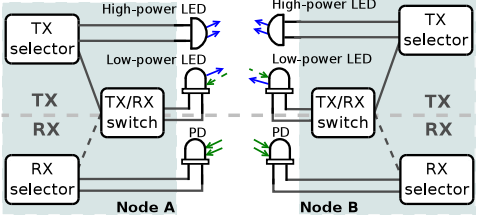
\includegraphics[scale=0.6]{images/diagram_cape_OpenVLC.png}
    \legend{Fonte: \citeonline{OpenVLCB}}
    \label{figura:diagramaVLC}
  \end{minipage}
  \hfill
  \begin{minipage}{0.4\textwidth}
    \centering
    \caption{Foto do hardware do OpenVLC} \label{fig_minipage_imagem1}
    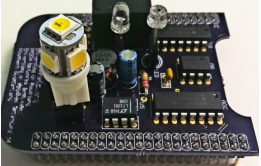
\includegraphics[scale=0.8]{images/Cape.png}
    \legend{Fonte: \citeonline{OpenVLCB}}
  \end{minipage}
\end{figure}

